\documentclass{beamer}

\usepackage[fontset=none]{ctex}
\usepackage{metalogo}
\usepackage{listings}
\usepackage{geometry}
\usepackage[shortlabels]{enumitem}
\usepackage{fancyvrb}
\usepackage{graphicx}
\usepackage{cancel}

\lstset{language=TeX,
    breaklines,
    basicstyle=\ttfamily,
    columns=flexible,
    numbers=left,
    numberstyle=\tiny,
    keywordstyle=\color{blue!70},
    commentstyle=\color{red!50!green!50!blue!50},
    frame=shadowbox,
    rulesepcolor=\color{red!20!green!20!blue!20}
}

\setCJKmainfont[BoldFont={FZCSJ.otf},
    ItalicFont={FZKTJ.otf},
    BoldItalicFont={FZCKJ.otf}]{FZSSJ.otf}
\setCJKsansfont[AutoFakeSlant,AutoFakeBold]{FZHTJ.otf}
\setCJKmonofont{FZFSJ.otf}

\AtBeginSection[]{
    \begin{frame}
        \tableofcontents[currentsection,hideallsubsections]
    \end{frame}
}

\usetheme{Warsaw}
\usefonttheme[onlymath]{serif}

\title{高速\LaTeX{}入门课程}
\author{曾梦辰}
\institute{北京师范大学OM学社}
\date{最后编译:\ \today}

\begin{document}
\maketitle

\begin{frame}
    \frametitle{目录}
    \tableofcontents
\end{frame}

\section{前言}

\begin{frame}
    \frametitle{关于\LaTeX{}}
    LaTeX (读作Lah--tek或Lay--tek, 不要读成Lay--teks), 是一种基于TeX的排版系统, 由美国计算机科学家Leslie Lamport在20世纪80年代初期开发.
    利用这种格式系统的处理, 即使用户没有排版和程序设计的知识也可以充分发挥由TeX所提供的强大功能, 不必一一亲自去设计或校对, 能在几天, 甚至几小时内生成很多具有书籍质量的印刷品生成复杂表格和数学公式, 这一点表现得尤为突出.
    因此它非常适用于生成高印刷质量的科技和数学, 物理文档.
    这个系统同样适用于生成从简单的信件到完整书籍的所有其他种类的文档.

    LaTeX使用TeX作为它的格式化引擎, 当前的版本是\LaTeXe.\pause

    \vspace{1cm}
    以上是抄的维基百科.
\end{frame}

\begin{frame}
    \frametitle{为什么要学\LaTeX{}?}
    工欲善其事, 必先利其器, 使用\LaTeX{}的\textbf{根本}目的是精确地排版大量数学公式.
    所以如果满足以上两个条件其一的就可以使用\LaTeX{}:\pause
    (1) 写\textbf{数学} (物理, 建模\dots, etc.) 作业, 写笔记;
    \begin{figure}[h]
        \centering
        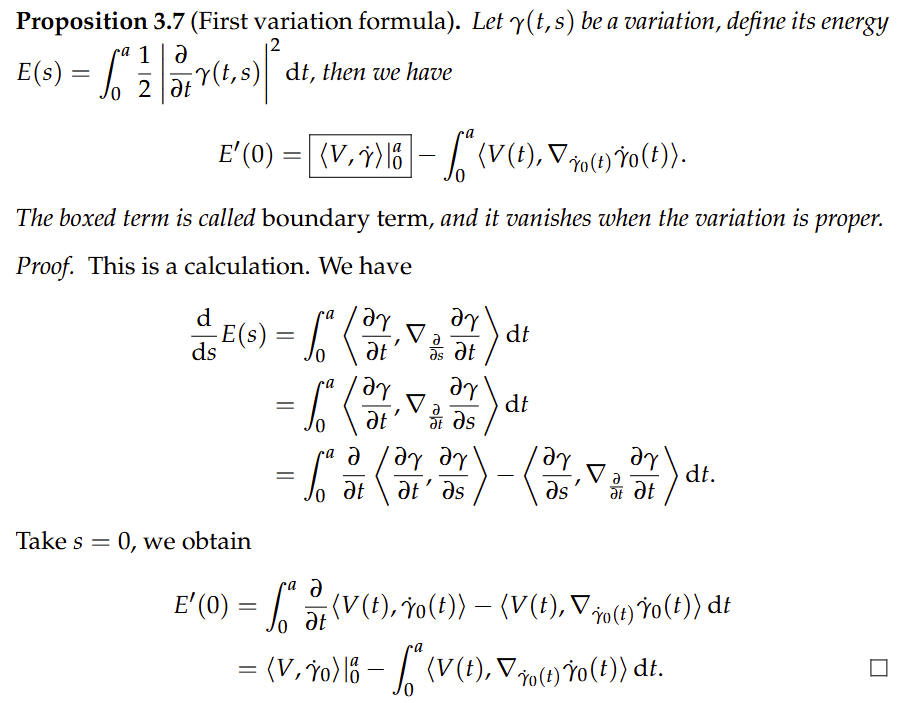
\includegraphics[width=0.6\textwidth]{figure/first-variation.png}
    \end{figure} 
\end{frame}

\begin{frame}
    (2) 对排版要求很高的文档.\pause

    当然, 要用合适的工具完成合适的任务.
    如果是排版简单的文档, 可以使用Microsoft Word提高效率; 如果涉及到大量复杂的表格, 应该使用Microsoft Excel; 如果你对排版有着出版物一样的极端要求, 应该使用Adobe InDesign.
\end{frame}

\begin{frame}
    \frametitle{参考资料}
    我们推荐一些可以阅读的参考资料.\pause
    \begin{itemize}
        \item<2-> Overleaf.\ \emph{Learn LaTeX in 30 minutes}.
        (本幻灯片的主要参考资料, 不过没有汉语翻译.)
        \item<3-> Tobias Oetiker, et.~al.\ \emph{一份 (不太) 简短的\LaTeXe{}介绍}.
        (可能是最好的入门教材.)
        \item<4-> Frank Mittelbach, Ulrike Fischer.\ \emph{The \LaTeX Companion}, 3rd Edition.
        (将近两千页的大肥书, 可以挑着看, 不要试图看完.)
        \item<5-> 本幻灯片. 用法: 使用Acrobat或者你喜欢的PDF阅读器, 然后利用鼠标左键/鼠标滚轮/幻灯片右下角的按钮进行翻页.
    \end{itemize}
\end{frame}

\begin{frame}
    \frametitle{听完本次课程后, 你将会\dots}
    \begin{enumerate}[(1)]
        \setcounter{enumi}{-1}
        \item \emph{能够}科学使用搜索引擎.
        \item 学会如何使用\Verb|texdoc|命令或者在\Verb|CTAN|上查找宏包文档.
        \item 学会如何使用Overleaf或者\TeX{}Page进行\LaTeX{}写作.
        \item 学会编写属于自己的\emph{Hello, World!}文档.
        \item \emph{知道}怎么输入数学公式.
        \item 从我的群里薅走一些实用书籍.
    \end{enumerate}\pause
    我觉得这些就够了.
    学习\LaTeX{}不是听一次课就能学会的, 需要自己下来勤加练习.
    有了上面这几点, 我认为已经有了一个良好的开端.
\end{frame}

\begin{frame}
    \frametitle{搜索引擎和\Verb|texdoc|}
    \textbf{不要用百度}$\times\infty$.
    在国内目前对科研, 学习目的最友好的搜索引擎是必应.\footnote{微软快给我打钱.}
    在搜索时, 善用高级搜索选项:
    \begin{figure}[h]
        \centering
        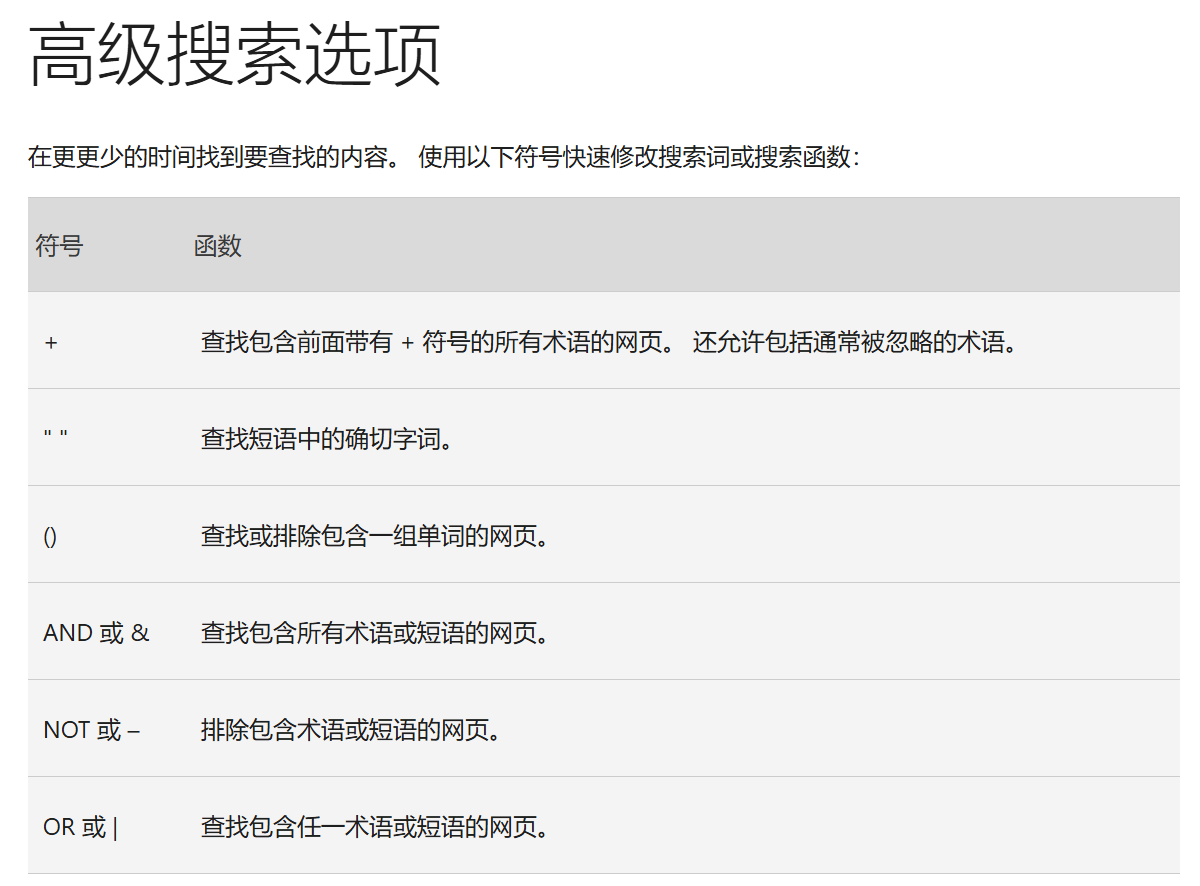
\includegraphics[width=0.65\textwidth]{figure/bing-search.png}
    \end{figure}
\end{frame}

\begin{frame}[fragile]
    \frametitle{搜索引擎和\Verb|texdoc|}
    如果你的电脑上安装了\TeX{}Live, 那么你可以在命令行中输入\Verb|texdoc Packagename|来查看名为\Verb|Packagename|的宏包的文档.
    如果没有安装的话, 可以在搜索引擎中搜索\Verb|CTAN Packagename|搜索宏包文档.\pause

    \textbf{练习1}: 使用\Verb|texdoc|或者在CTAN上找到文档\emph{lshort-chinese}.\\
    \textbf{练习2}: 搜索在\LaTeX{}中使用\Verb|bibtex|插入参考文献的办法 (你不必要现在学会), \textbf{排除}所有来自\xcancel{CSDN}的内容.
\end{frame}

\section{环境配置}

\begin{frame}
    \frametitle{\TeX{}Live的安装}
    这道题期末不考.\pause

    感兴趣的同学可以查看文档\emph{一份简短的关于\LaTeX{}安装的介绍} (\Verb|texdoc install-latex-guide-zh-cn|).
\end{frame}

\begin{frame}
    \frametitle{开始使用Overleaf}
    首先打开网址\url{https://cn.overleaf.com}, 看到如下页面:
    \begin{figure}[h]
        \centering
        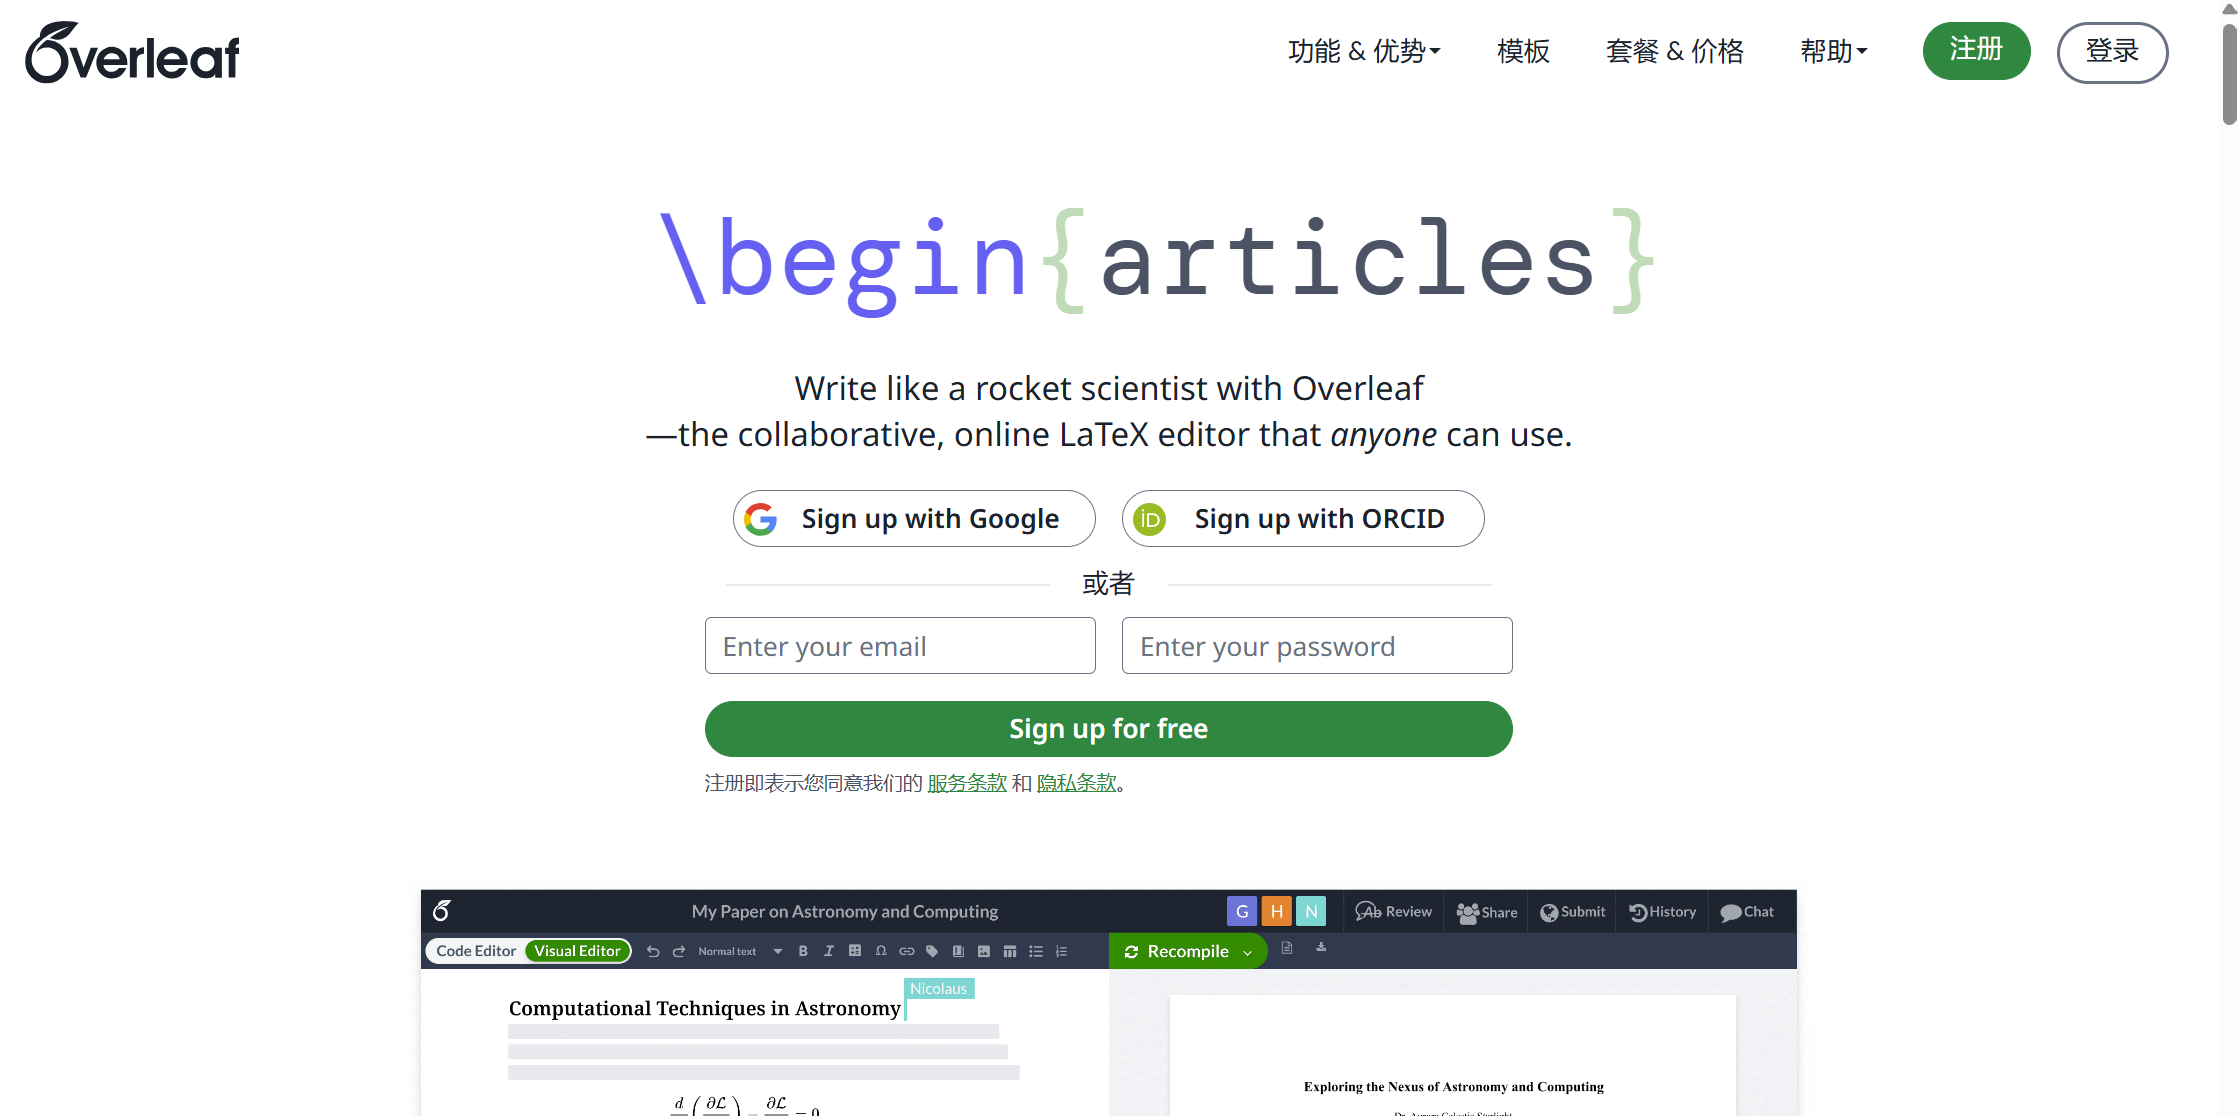
\includegraphics[width=0.8\textwidth]{figure/overleaf-signin.png}
    \end{figure}\pause
    然后在这两个方框里填写你的邮箱和你想要的密码.
    Then enjoy \LaTeX{ing}!
\end{frame}

\section{编写文档}

\subsection{我的Hello, world!}

\begin{frame}
    \frametitle{创建第一个项目}
    现在你创建好了账号, 你应该会看到这样一个页面:
    \begin{figure}[h]
        \centering
        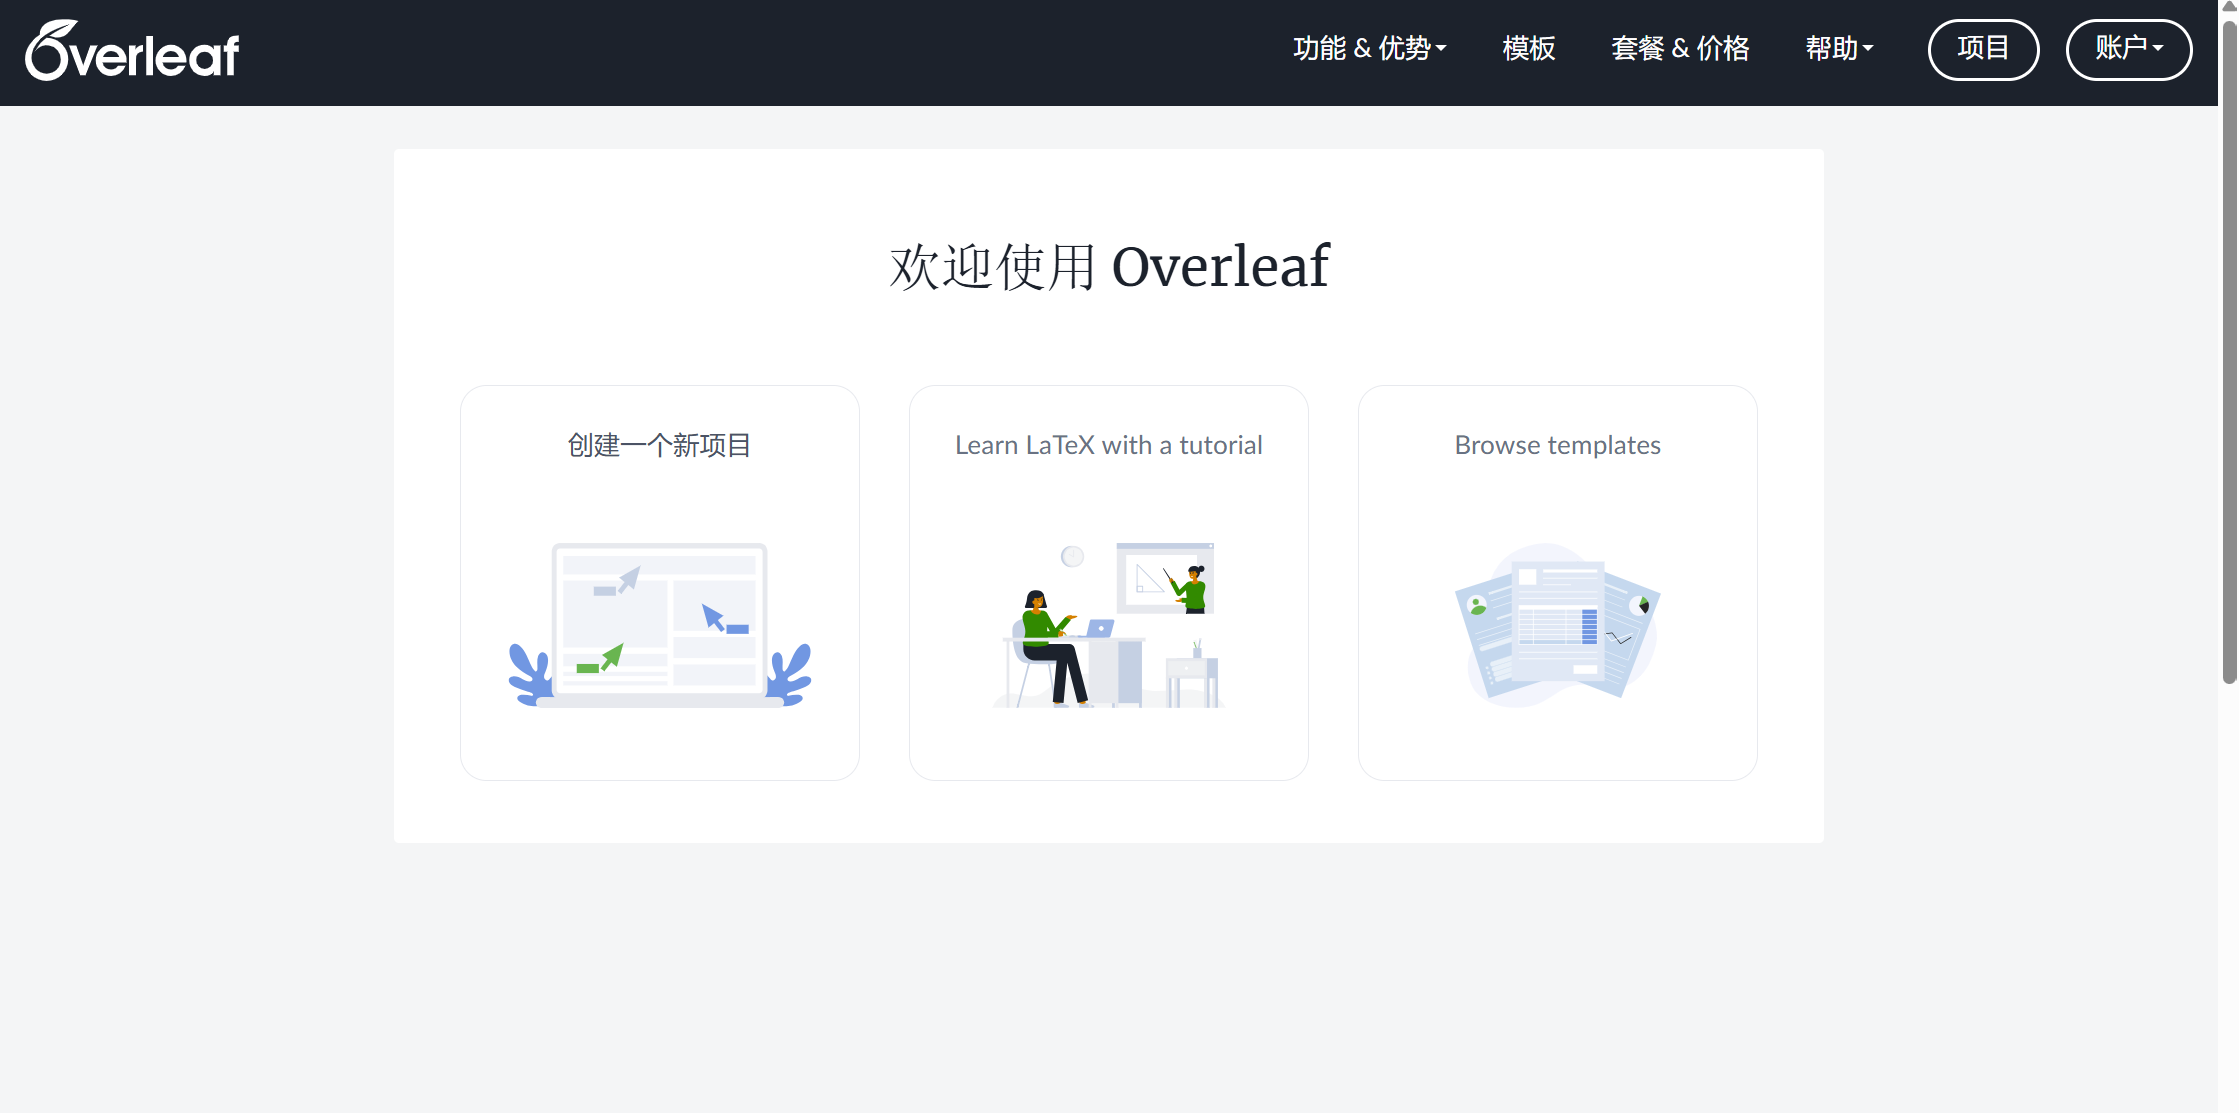
\includegraphics[width=0.8\textwidth]{figure/overleaf-startproject.png}
    \end{figure}\pause
    然后依次``创建一个新项目'', ``空白项目'', 并输入项目名称\Verb|Hello, world!|或者你喜欢的名字.\pause

    之后再创建项目的页面不长这样, 但是也很容易操作.
\end{frame}

\begin{frame}[fragile]
    \frametitle{编写Hello, world!的代码}
    把Overleaf自带的代码全部删掉, 然后输入如下的代码: (请注意所有标点都是英文标点)
    \begin{lstlisting}
        \documentclass[12pt]{article}
        \usepackage[paper=a4paper]{geometry}
        \title{Hello, World!}
        \author{Your name\thanks{ID: Your ID}}
        \date{\today}
        \begin{document}
            \maketitle
            Hello, world! Hello, \LaTeX!
        \end{document}
    \end{lstlisting}
    或者直接复制粘贴我群里发的代码.
\end{frame}

\begin{frame}
    \frametitle{一个好习惯}
    点击左上角``菜单'', 然后如图将编译器调整为\XeLaTeX{}.
    \begin{figure}[h]
        \centering
        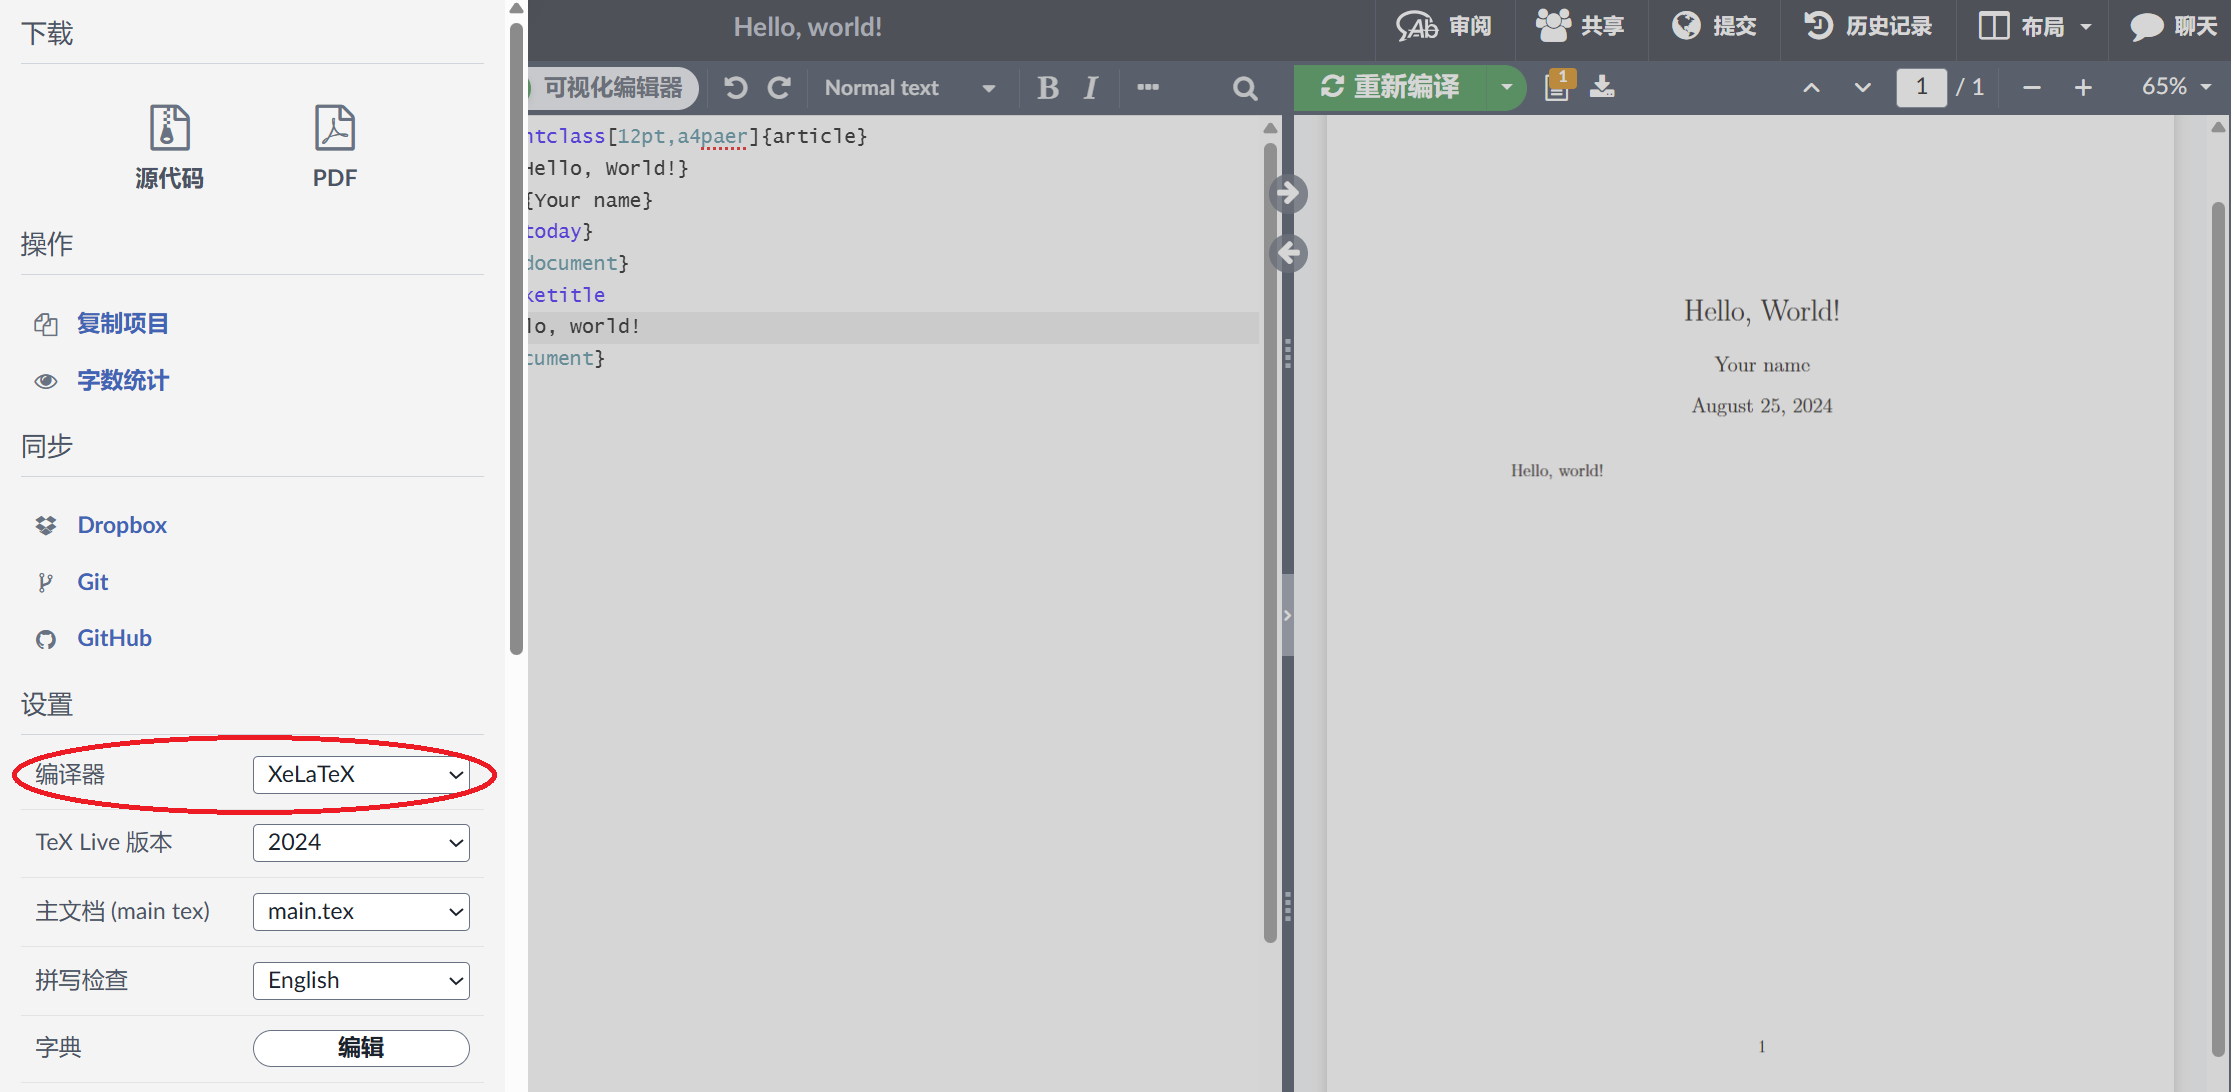
\includegraphics[width=0.8\textwidth]{figure/overleaf-compiler.png}
    \end{figure}
    然后可以点``重新编译''查看效果.

    使用Overleaf的好处是你不用操心编译, 直接点``重新编译''就可以了.
\end{frame}

\begin{frame}[fragile]
    \frametitle{控制序列}
    我们开始讨论\LaTeX{}的语法.
    一个典型的\textbf{控制序列} (control sequence) 形如
    \begin{lstlisting}
        \csname[option]{#1}
    \end{lstlisting}
    其中\Verb|\csname|是控制序列的名称, 花括号内的是控制序列作用的对象, 方括号内是参数.
    有时候后两者是不必要的.
    我们现在见过了控制序列\Verb|\documentclass[12pt]{article}|等, 接下来我们会仔细讨论它们的含义.
\end{frame}

\begin{frame}[fragile]
    \frametitle{导言区}
    文档\Verb|Hello, World!|的导言区为
    \begin{lstlisting}
        \documentclass[12pt]{article}
        \usepackage[paper=a4paper]{geometry}
    \end{lstlisting}\pause
    简单的识别导言区的方法就是导言区在\Verb|\begin{document}|之前.
    在导言区中, 我们声明了\textbf{文档类}为\Verb|article|, 并\textbf{引用}了\Verb|geometry|包.
    文档类\Verb|article|指的是文档的类型为``文章'', 文档类的参数\Verb|12pt|是全局字体大小, 默认为10pt, 这里调成12pt是为了照顾大家的英语课.
    \Verb|geometry|包的参数\Verb|paper|指定了纸张大小为A4.\pause

    \textbf{练习}: 将字体大小调节为10pt与11pt, 并调节纸张大小为\Verb|b5paper|, 观察效果.
\end{frame}

\begin{frame}[fragile]
    \frametitle{正文}
    正文由\Verb|\begin{document}|与\Verb|\end{document}|包裹.
    在这之后的任何内容都会被编译器忽略.\pause

    正文中的\Verb|\maketitle|将产生标题 (页).
    在\LaTeX{}中, 在源代码里断行将会导致文章中断句, 而分段则通过在源代码中给出一个空行实现.
    建议无论使用什么语言写作, 都使用英文标点符号.
    
    \textbf{练习}: 在正文中输入以下代码, 并观察效果.
    \begin{lstlisting}
        \maketitle
        Hello, world!
        Hello, \LaTeX!

        This is my document.
    \end{lstlisting}
\end{frame}

\begin{frame}[fragile]
    \frametitle{标题, 作者与日期}
    观察以下五条控制序列:
    \begin{lstlisting}
        \title{Hello, World!}
        \author{Your name\thanks{ID: Your ID}}
        \date{\today}
    \end{lstlisting}
    其中\Verb|\title{}|指定文章的标题, \Verb|\author|指定作者, \Verb|\thanks{}|提供作者的信息, \Verb|\date{}|指定日期, 而\Verb|\today|则输出当前的日期.
\end{frame}

\begin{frame}[fragile]
    \frametitle{输入中文}
    直接在\LaTeX{}里输入中文是做不到的, 我们需要使用一些宏包或者文档类.
    我们可以在导言区引用\Verb|ctex|包
    \begin{lstlisting}
        \usepackage{ctex}
    \end{lstlisting}
    或者直接使用\Verb|ctexart|文档类 (中文文章文档类.)
    \begin{lstlisting}
        \documentclass{ctexart}
    \end{lstlisting}
    \pause

    \textbf{提示1}: 一定要使用\XeLaTeX{}编译.\pause

    \textbf{提示2}: 课下你可能会找到某些告诉你使用\Verb|CJK|包或者\Verb|cctart|文档类输入中文的资料, 这是\textbf{过时的}, 一定不要学.\pause

    \textbf{练习}: 引用\Verb|ctex|包, 然后在你刚才的文档里随便输入一些中文试试.
\end{frame}

\subsection{输入数学公式}
\begin{frame}[fragile]
    \frametitle{输入数学公式}
    现在流行的数学公式输入宏包是来自美国数学会的\Verb|amsmath|宏包.
    新建一个项目 (这个应该都会了吧), 然后在导言区输入
    \begin{lstlisting}
        \usepackage{amsmath}
        \usepackage{amssymb}
        \usepackage{amsthm}
    \end{lstlisting}
    (请记得补充完整文档类, 标题和\Verb|\maketitle|)
    这三个宏包依次提供AMS数学环境, 更多的符号和定理环境.
    然后在正文输入
    \begin{lstlisting}
        We have Pythagorean theorem $a^2+b^2=c^2$ and fundamental theorem of calculus
        \[\int_a^bf'(x)dx=f(b)-f(a)\]
        provided $f'(x)$ is Riemann integrable.
    \end{lstlisting}
\end{frame}

\begin{frame}[fragile]
    \frametitle{数学公式: 语法}
    数学公式分为两种, 一种是\emph{行内公式}, 另一种是\emph{行间公式}, 分别使用\Verb|$...$|和\Verb|\[...\]|包裹.
    也有使用\Verb|\(...\)|包裹行内公式和使用\Verb|$$...$$|包裹行间公式的, 但这两种写法我个人不推荐.

    在上一页的公式中, 我们见到了\Verb|a^b|表示上标.
    而下标则通过\Verb|a_b|表示.
    \Verb|\int|则是\emph{算符}, 它会作用在一些公式上.
    \Verb|amsmath|宏包提供了很多常见函数, 例如下面的例子:
    \begin{lstlisting}
        傅里叶分析中的狄利克雷核为
        \[\sum_{n=-N}^{N}e^{inx}=\frac{\sin(N+\frac{1}{2})x}{\sin(x/2)}\]
    \end{lstlisting}
    (记得引\Verb|ctex|包哦$\sim$)
\end{frame}

\begin{frame}[fragile]
    \frametitle{数学公式: 语法}
    在上一页的公式中, 要注意花括号和算符的作用.
    请尝试编译以下代码并观察效果.
    \begin{lstlisting}
        \[e^ix=cos(x)+isin(x)\]
        \[e^{ix}=\cos(x)+i\sin(x)\]
    \end{lstlisting}

    事实上, \TeX{}引擎编译时的实际过程是逐字符展开, 一个控制序列实际上是一系列字符的组合, 而花括号形成一个``组'', 并被视为一个字符.\pause

    回到上一页的公式, 我们见到了表示分式的\Verb|\frac{}{}|.
    与分式类似的有根式\Verb|\sqrt[]{}|.
    请编译以下代码并观察效果.
    \begin{lstlisting}
        方程$x^n=a$ ($a>0$) 的$n$个复根为
        \[x_k=\sqrt[n]{a}(\cos\frac{2k\pi}{n}+i\sin\frac{2k\pi}{n}).\]
    \end{lstlisting}
\end{frame}

\begin{frame}
    \frametitle{学习数学公式输入}
    受到篇幅和课时限制, 本幻灯片不可能面面俱到地讲授\LaTeX{}的公式输入.
    所以我们应当阅读一些书籍, 例如我们提到的\emph{一份 (不太) 简短的\LaTeXe{}介绍}.
    接下来我们通过阅读学习一些\LaTeX{}公式输入技巧.\pause

    现在请阅读4.3.9小节, 并重新输入上一页的公式:
    \[x_k=\sqrt[n]{a}\left(\cos\frac{2k\pi}{n}+i\sin\frac{2k\pi}{n}\right)\]
    \textbf{提示}: 我们这里使用了\emph{定界符}来控制括号的大小.
\end{frame}

\begin{frame}[fragile]
    \frametitle{学习数学公式输入}
    现在请阅读4.5节, 并输入下面的矩阵公式:
    \begin{align*}
        &\frac{d}{dx}\left(\det\left[\begin{array}{ccc}
            f_{11}(x) & \cdots & f_{1n}(x)\\
            \vdots & \ddots & \vdots \\
            f_{n1}(x) & \cdots & f_{nn}(x)
        \end{array}\right]\right)\\
        =&\sum_{i=1}^n\det\left[\begin{array}{ccccc}
            f_{11}(x) & \cdots & f'_{1i}(x) & \cdots & f_{1n}(x)\\
            \vdots & \ddots & \vdots & \ddots & \vdots \\
            f_{n1}(x) & \cdots & f'_{ni}(x) & \cdots & f_{nn}(x)
        \end{array}\right]
    \end{align*}
    输入的时候不需要考虑换行, 直接输入即可.

    可能会用到的符号: 行列式\Verb|\det|, 横省略号$\cdots$\Verb|\cdots|, 竖省略号$\vdots$\Verb|\vdots|, 斜省略号$\ddots$\Verb|\ddots|.
\end{frame}

\begin{frame}[fragile]
    \frametitle{数学符号表}
    在\Verb|lshort-chinese|中, 第4.9节为数学符号表.
    请对照数学符号表输入以下公式:
    \[\Gamma^\alpha_{\beta\gamma}=\frac{1}{2}g^{\alpha\nu}(\partial_\beta g_{\nu\gamma}+\partial_\gamma g_{\beta\nu}-\partial_\nu g_{\beta\gamma}).\]
    以及
    \[\operatorname{Vol}(B_r(p))=\omega_nr^n\left(1-\frac{\operatorname{Scal}(p)}{6(n+2)}r^2+O(r^3)\right)\quad(r\to 0).\]
    \textbf{提示}: $\operatorname{Vol}$与$\operatorname{Scal}$是算符, 请用\Verb|\operatorname{}|包裹它们.
    可以用\Verb|\quad|制造一个较长的空格.
    \pause

    \Verb|lshort-chinese|中的符号表是一个比较小 (但是够用) 的符号表, 完整的符号表请使用\Verb|texdoc|或者CTAN查找文档\Verb|symbols| (完整名称为\emph{The Comprehensive \LaTeX{} Symbol List}).
\end{frame}

\subsection{一个完整的例子}

\begin{frame}
    \frametitle{一个完整的例子}
    请再次新建一个项目 (这次你可以不删代码), 我们的目标是尽可能地输出如图的文档 (纸张要求为B5).
    \begin{figure}[h]
        \centering
        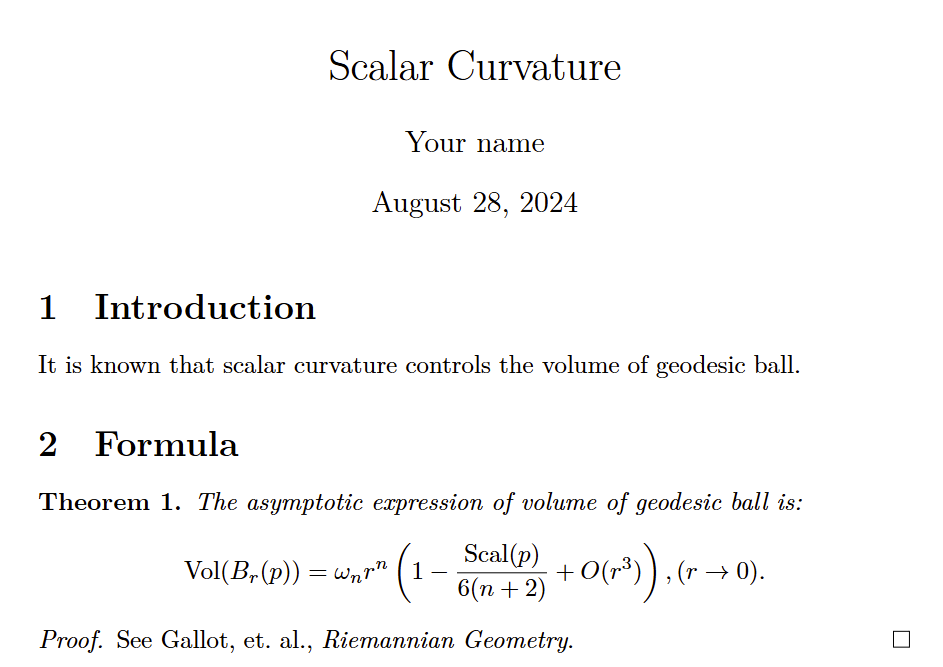
\includegraphics[width=0.7\textwidth]{figure/example.png}
    \end{figure}
\end{frame}

\begin{frame}[fragile]
    \frametitle{文档结构}
    \Verb|article|文档类提供了从高到低\Verb|\section|, \Verb|\subsection|, \Verb|\subsubsection|三个层次的章节.
    如果你之后可能会用到\Verb|book|文档类的话, 最高还有一个\Verb|\chapter|章节层级.

    在你需要的位置可以放置\Verb|\tableofcontents|生成目录.

    \textbf{练习}: 随便打开一个项目, 然后设置小节并生成目录.
\end{frame}

\begin{frame}
    \frametitle{字体控制}
    \LaTeX{}中提供了控制字体类型的命令.
    具体使用如下表:
    \begin{figure}[h]
        \centering
        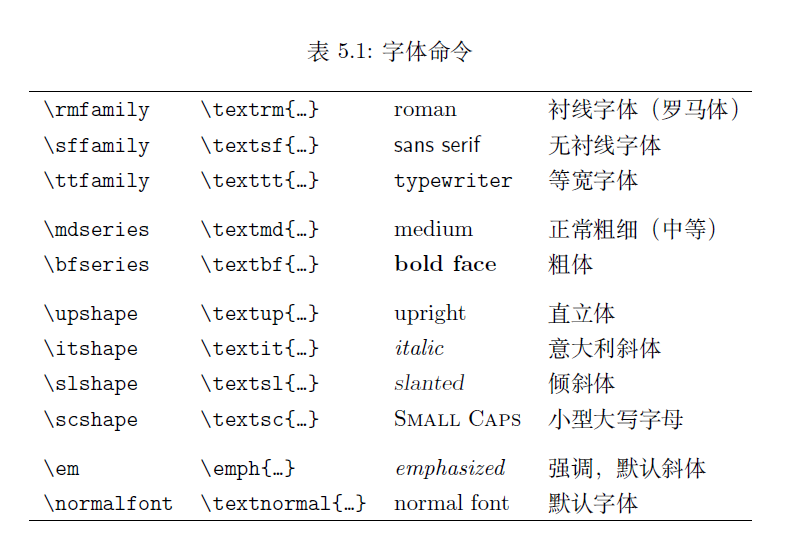
\includegraphics[width=0.7\textwidth]{figure/lshort-fonts.png}
    \end{figure}
\end{frame}

\begin{frame}[fragile]
    \frametitle{字体控制}
    有些同学可能有使用\textrm{Times}类字体的需求, 这里提供两种解决方案:\\
    (1) 使用\Verb|fontspec|宏包, 一个最小工作示例是
    \begin{lstlisting}
        \usepackage{fontspec}
        \setmainfont{Times New Roman}
    \end{lstlisting}
    注意使用\Verb|fontspec|包的话必须使用\XeLaTeX{}编译.\\
    (2) 使用\Verb|newtxtext|与\Verb|newtxmath|宏包.
    这将同时改变你的正文字体与数学字体.
\end{frame}

\begin{frame}[fragile]
    \frametitle{定理环境}
    \Verb|amsthm|包中提供了声明定理环境的方法.
    一个例子如下:
    \begin{lstlisting}
        \theoremstyle{plain}
        \newtheorem{theorem}{Theorem}
    \end{lstlisting}
    其中\Verb|\theoremstyle{}|决定了接下来声明的定理环境的风格, 有plain, definition和remark三种选择.
    \Verb|\newtheorem{}{}|则声明了定理环境, 前一个参数表示控制序列的名称, 后一个参数则表示显示的名称.
    例如, 在以上代码声明了\Verb|Theorem|环境之后, 可以通过代码
    \begin{lstlisting}
        \begin{theorem}
            Scalar curvature\dots
        \end{theorem}
    \end{lstlisting}
    来使用\Verb|Theorem|环境.
\end{frame}

\begin{frame}[fragile]
    \frametitle{证明环境}
    \Verb|amsmath|包中也提供了证明环境, 使用\Verb|\begin{proof}|与\Verb|\end{proof}|包裹即可.
    例如
    \begin{lstlisting}
        \begin{proof}
            We have Ricci identity
            \[\nabla_{Y,X}T-\nabla_{X,Y}T=R(X,Y)T\]
        \end{proof}
    \end{lstlisting}
\end{frame}

\begin{frame}
    \frametitle{一个完整的例子}
    现在你应该可以完成这个练习了.
    \begin{figure}[h]
        \centering
        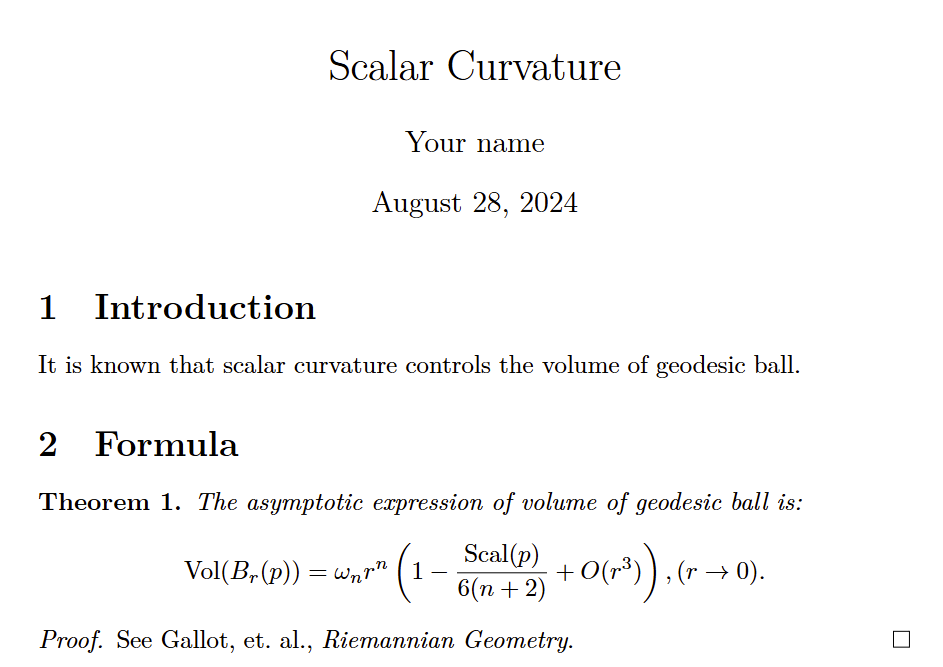
\includegraphics[width=0.7\textwidth]{figure/example.png}
    \end{figure}
\end{frame}

\subsection{使用模板}

\begin{frame}
    \frametitle{使用模板}
    请打开Overleaf, 自行摸索搜索模板 (template) 的方式, 然后找到``BNU课程论文模板''.
    此后, 学习使用该模板并重新完成上面的例子. (注意效果肯定会发生变化)
    \begin{figure}[h]
        \centering
        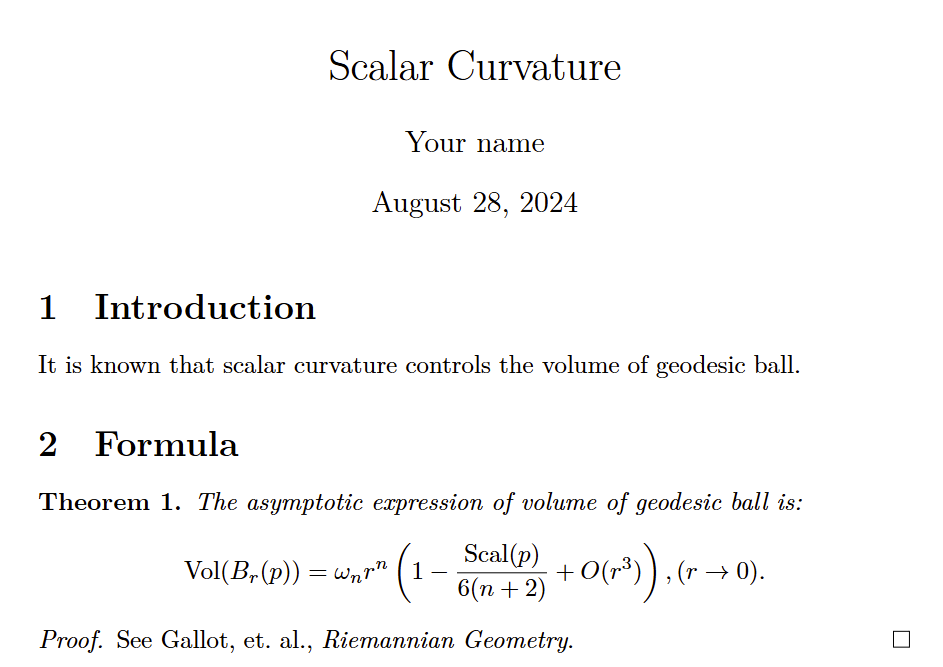
\includegraphics[width=0.7\textwidth]{figure/example.png}
    \end{figure}
\end{frame}

\subsection{调试}

\begin{frame}
    \frametitle{调试}
    调试, 或者说debug, 是写\LaTeX{}时不可避免会遇到的修正错误的过程.

    请大家将压缩包中的\Verb|debug.zip|上传至Overleaf (新建项目--上传项目), 然后编译, 看看会发生什么.
    接下来请大家和我一起debug.

    再次提醒一个好习惯: 请务必在代码中分行, 也即一行只写一句话, 这对debug大有裨益.
\end{frame}

\section{结束语}

\begin{frame}
    \frametitle{最后的话}
    最后我想说
    \begin{itemize}
        \item<2-> 首先不要害怕使用\LaTeX{}, 虽然\LaTeX{}上手确实不容易, 但是对着书籍和搜索引擎边用边改也是能够入门的.
        \item<3-> 请一定要去阅读\emph{一份 (不太) 简短的\LaTeXe{}介绍}, 即使没有时间全部读完也要挑着重点读.
        \item<4-> 善用搜索引擎, 可以试试AI\dots?
        \item<5-> 实在不行了就多问师兄师姐. 直接找我装\TeX{}Live都是可以的.
    \end{itemize}
\end{frame}

\begin{frame}
    \Huge{\centerline{感谢聆听!}}
\end{frame}

\end{document}